\chapter{Ideation}\label{ideation}

This chapter exposes the ideation phase of the design process. By
looking at canonical examples and solutions to conceptually similar
problems, lessons are learned to support the ideation. A series of
different concepts is sketched out, which ultimately leads to the design
chosen for prototyping.

\section{Canonical Examples}\label{similar}

The most ubiquitous visualization of program structure is probably
\emph{syntax highlighting} or \emph{syntax colouring}. This concept aims
to make the developer distinguish entities of the programming language
by showing them in different font weights, styles, or colours. According
to the survey results (see chapter \fullref{exploration}), syntax
highlighting can help with a number of different problems: recognizing
errors and typos, distinguishing language constructs from variables and
values, and orienting through specific visual patterns (compare also
\citeasnoun{deline}). Figure \ref{fig:syntaxhighlighting} shows syntax
highlighting in an \ac{html} document; HTML elements are printed in
blue, whereas attributes are printed in purple, values in red, comments
in yellow, and content in black.

\begin{figure}[htbp]
\centering
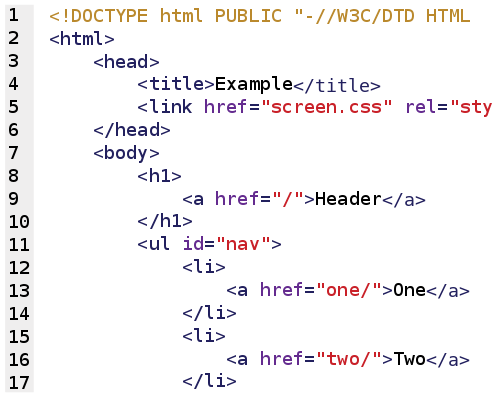
\includegraphics[keepaspectratio,width=0.75\textwidth]{img/syntax_highlighting.png}
\caption{Syntax highlighting in an HTML document}
\label{fig:syntaxhighlighting}
\end{figure}

In his talk „Monads and Gonads“, \citename{crockford} presents an
alternative to syntax highlighting which he calls „context colouring“
\citeyear{crockford}. Instead of using font styles and colours in order
to highlight different elements of the \emph{syntax}, he instead
highlights different \emph{scopes}. Figure \ref{fig:contexthighlighting}
illustrates this concept: The global scope is presented in white,
whereas nested scopes are marked green, yellow and blue, respectively.
In this concrete example, identifiers are always coloured in the colour
of the scope of \emph{where they were defined}. For example, the
appearance of \texttt{value} in the innermost scope is yellow, the
colour of the scope in which \texttt{value} was declared (as a function
parameter to the function \texttt{unit}).

\begin{figure}[htbp]
\centering
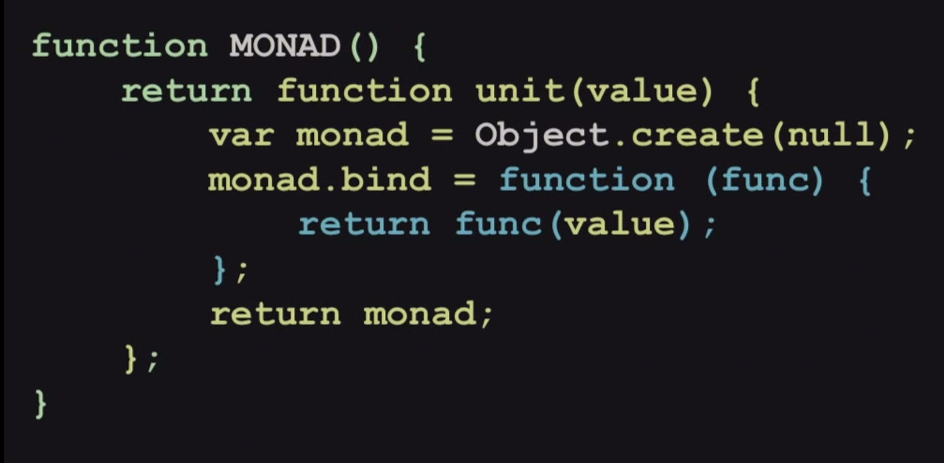
\includegraphics[keepaspectratio,width=0.75\textwidth]{img/context.png}
\caption{Context colouring in JavaScript, as proposed by Crockford (2013)}
\label{fig:contexthighlighting}
\end{figure}

\textbf{Theseus} is a JavaScript debugger built as a plug-in for the
Brackets IDE. It integrates with the code editor itself and shows
information inline, in the gutter and in a panel on the bottom of the
Brackets window (see Figure \ref{fig:theseus}). Theseus is mostly used
for asynchronous debugging, so the way those UI elements are used
corresponds to this purpose. For every function definition, Theseus
shows (in the gutter) the number of times the function has been called.
Functions that have never been called are marked with a grey background
in the source code. Additionally, the panel on the bottom shows
information about the function the cursor is positioned
in\footnote{It shows asynchronous call stacks, which are not of relevance to this thesis.}.

\begin{figure}[htbp]
\centering
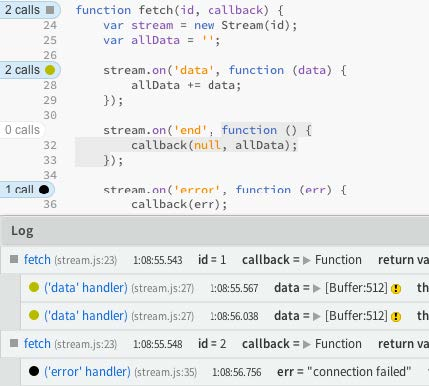
\includegraphics[keepaspectratio,width=0.5\textwidth]{img/theseus.jpg}
\caption{Theseus’ asynchronous JavaScript debugging (Lieber et al. 2014)}
\label{fig:theseus}
\end{figure}

\textbf{JSHint} is a so-called \emph{linting} tool, or \emph{linter},
for JavaScript: it detects bad programming practices (\emph{code
smells}) by checking JavaScript code against a set of rules, and
therefore tries to prevent common problems. Originally built as a
command-line tool, JSHint is implemented in many IDEs through the
respective plug-in systems. The \emph{Sublime Linter} plug-in\footnote{See
  \url{http://www.sublimelinter.com/}} for Sublime Text 3 implements
JSHint (and other linting tools) \emph{inline}: hints of bad code or
inconsistent style are shown in the text editor itself and are indicated
in the gutter. If the cursor is on top of problematic code, the
respective hint is printed in the status bar. \emph{Sublime Linter}
behaves according to the characteristics identified before: it is
modular, as linters for different programming languages can be
plugged-in; it is lightweight and does not slow the editor down; it
focuses on code by displaying results inline without cluttering the
editor window; and it is smart to some extent, as it allows the
configuration of certain programming guidelines. The prototype presented
later in this thesis borrows many characteristics and design decisions
from linting tools such as this one. This is due to the fact that both
the problem of code smells and the problem of scope can mostly be solved
with static analysis and presented in a similar manner.

\begin{figure}[H]
\centering
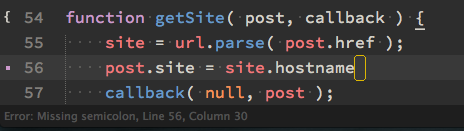
\includegraphics[keepaspectratio,width=0.6\textwidth]{img/jshint.png}
\caption{Sublime Linter indicating an error on line 56 (the semicolon is missing). The error is shown inline, in the gutter, and in the status bar.}
\label{fig:sublimelinter}
\end{figure}

In terms of navigating and displaying tree structures in relation to the
actual source code, the \emph{Element Inspector} of \textbf{Chrome
Developer Tools} makes a good example (see Figure \ref{fig:devtools}).
The structure of \acs{html} is quite similar to that of scope, as it is
nested in the same way, which is why ideas can be taken from the
Developer Tools. They show the source code of the inspected website and
allows the user to select any \acs{html} element within. In the other
parts of the window, information relevant to the selected element is
shown.

\begin{figure}[htbp]
\centering
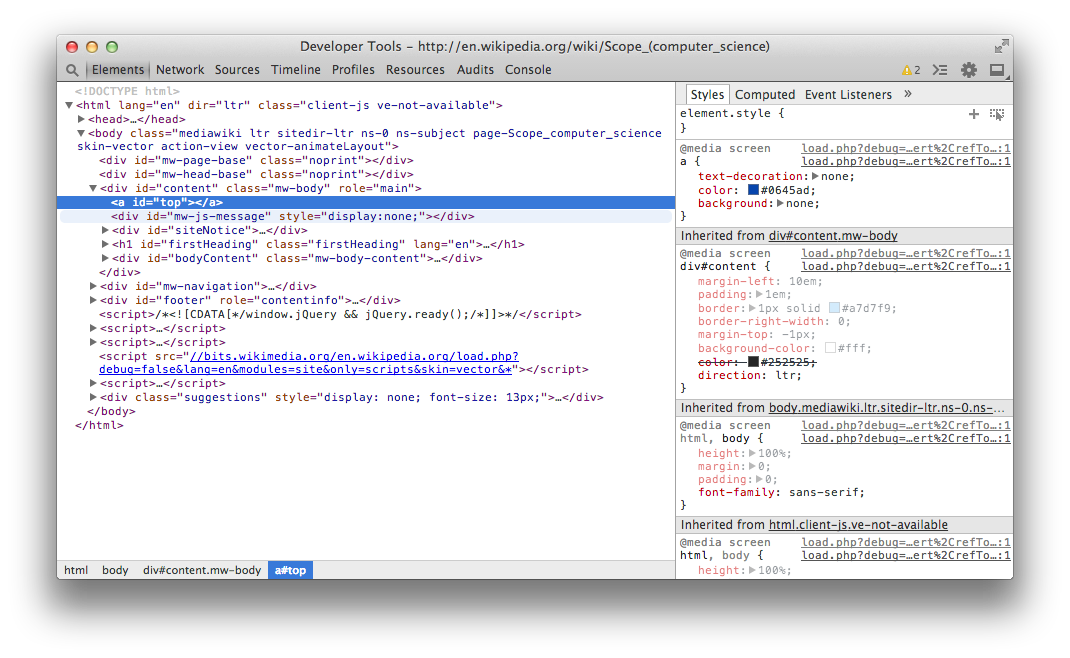
\includegraphics[keepaspectratio,width=\textwidth,height=0.75\textheight]{img/devtools.png}
\caption{Chrome Developer Tools with Element Inspector}
\label{fig:devtools}
\end{figure}

At the bottom of the window, a status bar shows the nesting of the
selected element: on the visual left (and logical top of the tree) is
the \texttt{html} element, inside it the \texttt{body}, then a
\texttt{div} and finally the selected \texttt{a} element. This status
bar can be used to navigate around the nested elements by clicking on
them. Clicking on the \texttt{body} element, for instance, highlights it
in the source code as well, and shows different style information on the
right-hand side.

Placed to the right of the source code is a sidebar. While it contains a
tabbed interface to browse different facets of the selected element, the
one that is relevant—\emph{Style}— is in focus on the screenshot. The
way that \ac{css} are applied to HTML elements is similar to the way
nested scope works: style that is defined on the ancestor elements may
influence the style of the selected element, which is why the relevant
styles are listed in order of precedence. The style rules that apply
with the highest precedence are listed on top, while the rules with the
lowest precedence are listed on the bottom. Style rules that are
overriden by rules of higher precedence are striked through, to indicate
that they do not apply anymore. This way of visualizing and organizing
information about nested structures is further used in the following
concept and design phases (see section \ref{concept-generation} and
chapter \ref{design}).

\section{Concept Generation}\label{concept-generation}

To support the ideation phase, existing \ac{ui} components used within
IDEs, as presented in chapter \ref{research}, were collected. Those
components were written down on post-it notes and used as seeds for
\emph{seeded brainstorming}: for each of the components, a set of
solutions should be developed that are similar, related to or based on
the respective component. Most of the ideas that resulted from the
brainstorming session make use of multiple components, for example the
\emph{scope chain} which is described further down: it made use of a
status bar as well as the code editor.

Some ideas of the brainstorming phase made it into first sketches.
Depending on the involved components, the sketching took two different
approaches. For ideas that used the code editor, it was important to
work with real, functioning code. Therefore, two JavaScript applications
were created to serve as examples:

\begin{itemize}
\itemsep1pt\parskip0pt\parsep0pt
\item
  A small web server application, that parses a markdown-formatted text
  file and renders it into an HTML template. The application runs on
  Node.js and represents a typical control flow for a blogging engine
  (i.e. content + template = site).
\item
  A client-side script (runs in a web browser) that fetches JSON data
  and presents them on a website, by the click of a button. This script
  represents typical client-side UI code, connecting a button event to a
  function and presenting the result in the UI.
\end{itemize}

The two applications were written in different styles: the server-side
application decouples its tasks by putting them into specific, named
functions (as far as it was seen appropriate) and therefore has a
relatively flat scope tree. In contrast, the client-side application
nests all function definitions inside each other, resulting in nearly
one function definition on each line, and far deeper indentation (in
other words, higher code complexity and deeply nested scope). A good
solution for this design problem should address both of those cases.

Printouts of the two JavaScript files served as a basis for ideation of
concepts involving the code editor. However, for concept ideas that
would mainly work with other UI components, such as a sidebar, or such
concept ideas that would introduce new UI components, a blank notebook
was used for sketching. The source code of the two JavaScript programs
can be found in the appendix.

The following is a list of the concepts that have been assumed to be the
most promising.

\begin{description}
\item[Scope Chain]
A breadcrumb
view\footnote{In the Yahoo Design Pattern Library: \url{https://developer.yahoo.com/ypatterns/navigation/breadcrumbs.html}}
of the active scope chain, similar to that of a selector chain in an
HTML editor (see figure \ref{fig:devtools}). The scope chain, which
corresponds to the position of the cursor in the code, would be
displayed as \gls{breadcrumbs} in a status bar. By hovering over a scope
level breadcrumb, the corresponding source code of that scope would be
highlighted in the code editor. Clicking on a scope level would navigate
to the corresponding code, i.e. position the cursor to the top of the
scope block.
\item[Scope Graph]
Similar to a class browser, the scope graph represents a tree view of
the application’s scopes. The user can navigate the source code using
the scope graph. It could be implemented as a sidebar or in a panel.
\item[Scope Colouring]
Similarly suggested by \citeasnoun{crockford}, the source code can be
coloured depending on its scope level. Crockford’s variation is meant to
replace syntax highlighting; one could instead complement syntax
highlighting by colouring the background (as Theseus does, see section
\fullref{similar}), rather than the text—for example in different shades
of grey.
\item[Inspect Scope]
Comparable to the Chrome Developer Tools \emph{Inspect Element}
function, the user can right-click into the source code and choose
„Inspect Scope“, which opens a panel that shows global variables,
current local variables as well as the value of \texttt{this} (the
latter would be possible in a debugging environment, as \texttt{this} is
only available at run-time).
\item[Gutter Scope]
Any new scope created in the source code is indicated in the gutter.
Comparable to how Sublime Linter indicates errors (by placing a coloured
dot or square in the gutter), the boundaries of the scope (i.e. its
first and last line) are denoted by a coloured dot. For every scope
level, the colour of the dot is different, so that the user can easily
see how deeply nested the scope is at any given point.
\item[Quick Inspect]
Similar to the \emph{Quick Edit} feature of Brackets, the value of
\texttt{this} can be inspected inline. By right-clicking on any point in
the source code and choosing the context menu point „Quick Inspect“, an
area slides out inline (between two lines of source code), showing the
value of \texttt{this} and available scope variables. As with the
\textbf{Inspect Scope} concept, this would require to run in a debugging
context to have access to \texttt{this}.
\end{description}

\begin{figure}[htbp]
\centering
\includegraphics[keepaspectratio,width=\textwidth]{img/sketches.png}
\caption{Some of the sketches created during ideation}
\label{fig:sketches1}
\end{figure}

The concept chosen for prototyping is a combination of \textbf{scope
chain}, \textbf{scope colouring}, and \textbf{inspect scope}. The
\emph{scope chain} is adapted as described above. \emph{Scope colouring}
is implemented in terms of background colouring. The \emph{inspect
scope} concept is adapted by means of its panel. The next chapter,
\nameref{design}, opens up the exact design decisions made for each of
the elements.
